\documentclass[11pt]{article}
\usepackage{graphicx} % Required for inserting images
\usepackage[a4paper, total={7in, 10in}]{geometry}
\usepackage{hyperref}
\usepackage{float}
\usepackage{listings}
\usepackage{xcolor}

\definecolor{pastelyellow}{RGB}{255, 255, 224}
\definecolor{lightorange}{RGB}{255, 200, 150}
\definecolor{codegray}{rgb}{0.5,0.5,0.5}
\definecolor{codepurple}{rgb}{0.58,0,0.82}

\lstdefinestyle{mystyle}{
    backgroundcolor=\color{pastelyellow},  
    commentstyle=\color{olive},
    keywordstyle=\color{blue},
    basicstyle=\fontfamily{pcr}\small,
    numberstyle=\tiny\color{codegray},
    stringstyle=\color{codepurple},
    frame=single,
    rulecolor=\color{lightorange} 
}

\lstset{style=mystyle}

\title{Assignment 3: Socket Programming Group Chat}
\author{20235140 Boseong Lee}
\date{November 2024}

\begin{document}

\maketitle

\section{Node.js and library environment information}
\begin{itemize}
  \item Node.js version: 20.12.1
  \item React.js version: 18.3.1
  \item Nest.js version: 10.4.6
  \item Socket.io version: 4.8.0
\end{itemize}

This project uses mono-repo structure.

\texttt{packages/client} is the React.js client.
\texttt{packages/server} is the Nest.js server.
\texttt{packages/shared} is the shared library between client and server.

\section{Key Features}

\begin{figure}[ht!]
  \centering
  \frame{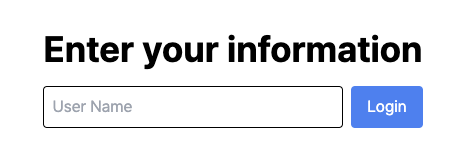
\includegraphics[width=7cm]{figures/01_login.png}}
  \caption{Login Screen}
  \label{fig:1}
\end{figure}

In login screen~\ref{fig:1} User can set their username appearing in the chat room.

\begin{figure}[H]
  \centering
  \frame{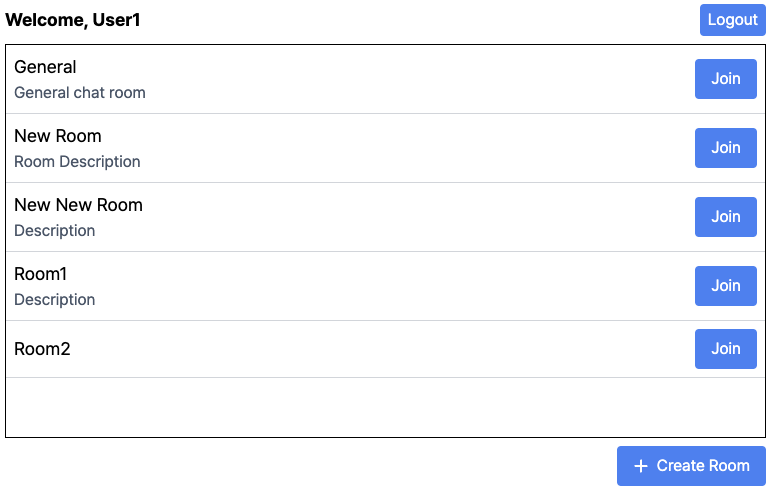
\includegraphics[width=10cm]{figures/02_list.png}}
  \caption{Chat Room List Page}
  \label{fig:2}
\end{figure}

In chat room list page~\ref{fig:2} User can see the list of chat rooms.
In header of the page, user can see the username set in the login screen and the \texttt{Logout} button to use another username.
Each chat room has the title, and description. Pressing the \texttt{Join} button will move to the chat room page.
User also can create a new chat room by pressing the \texttt{Create Room} button.

\begin{figure}[H]
  \centering
  \frame{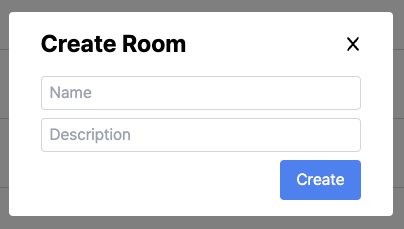
\includegraphics[width=8cm]{figures/03_create_room.png}}
  \caption{Creating Room}
  \label{fig:3}
\end{figure}

\texttt{Create Room} button will show the modal~\ref{fig:3} to create a new chat room.
User can set the title and description of the chat room.
After, pressing the \texttt{Create} button will create a new chat room.

This project uses \texttt{socket.io} to implement real-time chat feature.
When user create a new chat room, client sends \texttt{socket.io} event to the server to create a new chat room.
Then, server broadcasts the new chat room to all the clients except the user who created the chat room.
It makes all the clients to see the new chat room in real-time.

\begin{figure}[H]
  \centering
  \frame{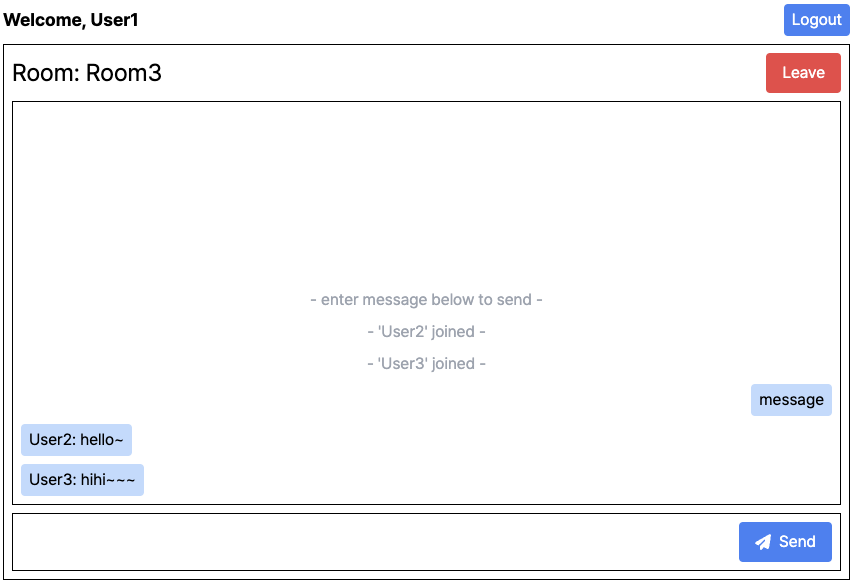
\includegraphics[width=12cm]{figures/04_chat_room.png}}
  \caption{Chat Room}
  \label{fig:4}
\end{figure}

When user joins the chat room, the user can see the chat messages~\ref{fig:4} in real-time.
User can send the message by typing in the input box and pressing the \texttt{Send} button.
The chat messages are shown in the chat room in real-time using \texttt{socket.io}.
Once user leaves the chat room, the user will not receive the chat messages from the chat room.
Also, there are system messages to notify the user joining and leaving the chat room.


\section{How to run the project}

This project uses \texttt{yarn berry} as a package manager.
Especially, this project uses mono-repo structure, so you need to run \texttt{yarn} in the root directory.
\texttt{yarn berry} can be installed by using \texttt{corepack} which is installed by \texttt{node.js} (\url{https://nodejs.org}).
After, you can run the project by following the steps below.

\begin{lstlisting}[language=bash]
$ npm install -g corepack  # if you don't have corepack installed
$ corepack enable

# Install dependencies
$ yarn install

# Run the server and client (run in different terminal)
$ yarn workspace server start
$ yarn workspace client dev
\end{lstlisting}

You can access the client at \texttt{http://localhost:5173}. The port number can be different.

\end{document}
